%%%%%%%%%%%%%%%%%%%%%%%%%%%%%%%%%%%%%%%%%%%%%%%%%%%%%%%%%%%%%%%%%%%%%%%%%%%%%%%%%%%%%%%%%%%%%%%%
%
% CSCI 1430 Project Progress Report Template
%
% This is a LaTeX document. LaTeX is a markup language for producing documents.
% Your task is to answer the questions by filling out this document, then to 
% compile this into a PDF document. 
% You will then upload this PDF to `Gradescope' - the grading system that we will use. 
% Instructions for upload will follow soon.
%
% 
% TO COMPILE:
% > pdflatex thisfile.tex
%
% If you do not have LaTeX and need a LaTeX distribution:
% - Departmental machines have one installed.
% - Personal laptops (all common OS): http://www.latex-project.org/get/
%
% If you need help with LaTeX, come to office hours. Or, there is plenty of help online:
% https://en.wikibooks.org/wiki/LaTeX
%
% Good luck!
% James and the 1430 staff
%
%%%%%%%%%%%%%%%%%%%%%%%%%%%%%%%%%%%%%%%%%%%%%%%%%%%%%%%%%%%%%%%%%%%%%%%%%%%%%%%%%%%%%%%%%%%%%%%%
%
% How to include two graphics on the same line:
% 
% \includegraphics[width=0.49\linewidth]{yourgraphic1.png}
% \includegraphics[width=0.49\linewidth]{yourgraphic2.png}
%
% How to include equations:
%
% \begin{equation}
% y = mx+c
% \end{equation}
% 
%%%%%%%%%%%%%%%%%%%%%%%%%%%%%%%%%%%%%%%%%%%%%%%%%%%%%%%%%%%%%%%%%%%%%%%%%%%%%%%%%%%%%%%%%%%%%%%%

\documentclass[11pt]{article}

\usepackage[english]{babel}
\usepackage[utf8]{inputenc}
\usepackage[colorlinks = true,
            linkcolor = blue,
            urlcolor  = blue]{hyperref}
\usepackage[a4paper,margin=1in]{geometry}
\usepackage{stackengine,graphicx}
\usepackage{fancyhdr}
\setlength{\headheight}{15pt}
\usepackage{microtype}
\usepackage{times}
\usepackage{booktabs}
\usepackage{float}

% From https://ctan.org/pkg/matlab-prettifier
\usepackage[numbered,framed]{matlab-prettifier}

\frenchspacing
\setlength{\parindent}{0cm} % Default is 15pt.
\setlength{\parskip}{0.3cm plus1mm minus1mm}

\pagestyle{fancy}
\fancyhf{}
\lhead{Final Project Proposal}
\rhead{CSCI 1430}
\rfoot{\thepage}

\date{}

\title{\vspace{-2cm}Final Project Proposal}


\begin{document}
\maketitle
\vspace{-3cm}
\thispagestyle{fancy}

\section*{Definitions}

\textbf{Team name: \emph{Super Zoom}}

\textbf{Team members: \emph{Michael Litt, Peter Huson, Gabe Weedon, Mary Dong}}

\section*{Project}
\begin{itemize}
  \item \textbf{What is your project idea?}
  
Our project idea is to perform super resolution up-sampling on images we provide. Super resolution up-sampling is performed by taking a low-resolution image as input, and using a neural network or heuristic model to output a higher resolution image with more details than the initial image. This can be accomplished through many different ways—--which we aim to explore in this project. We would like to explore where current state-of-the art algorithms and models perform well and where they perform poorly, then improve on the areas that need work. 

  \item \textbf{What data will you use?}
  
Currently, the best datasets for super-resolution (SR) models are the ones used in the annual NTIRE super-resolution challenge; these are described  \href{http://www.vision.ee.ethz.ch/~timofter/publications/Agustsson-CVPRW-2017.pdf}{here}. Specifically, we want to use the DIV2K dataset suggested by NTIRE, which has the following properties: (1) 1000 total images (800 train; 100 validation; 100 test) featuring a diverset set of content (animals, people, scenery, etc.) (2) All are 2K resolution (high resolution; can be blurred) (3) All are cropped to multiple of 12 pixels since the most common magnification factors for SR are $\times2$, $\times3$ and $\times4$. (4) Already preprocessed and downsampled so we can directly work with both low-res and high-res data. This dataset is easy to work with and allows us to compare our results with state-of-the-art models which are also trained and evaluated using the same data.
\begin{figure}[H]
    \centering
    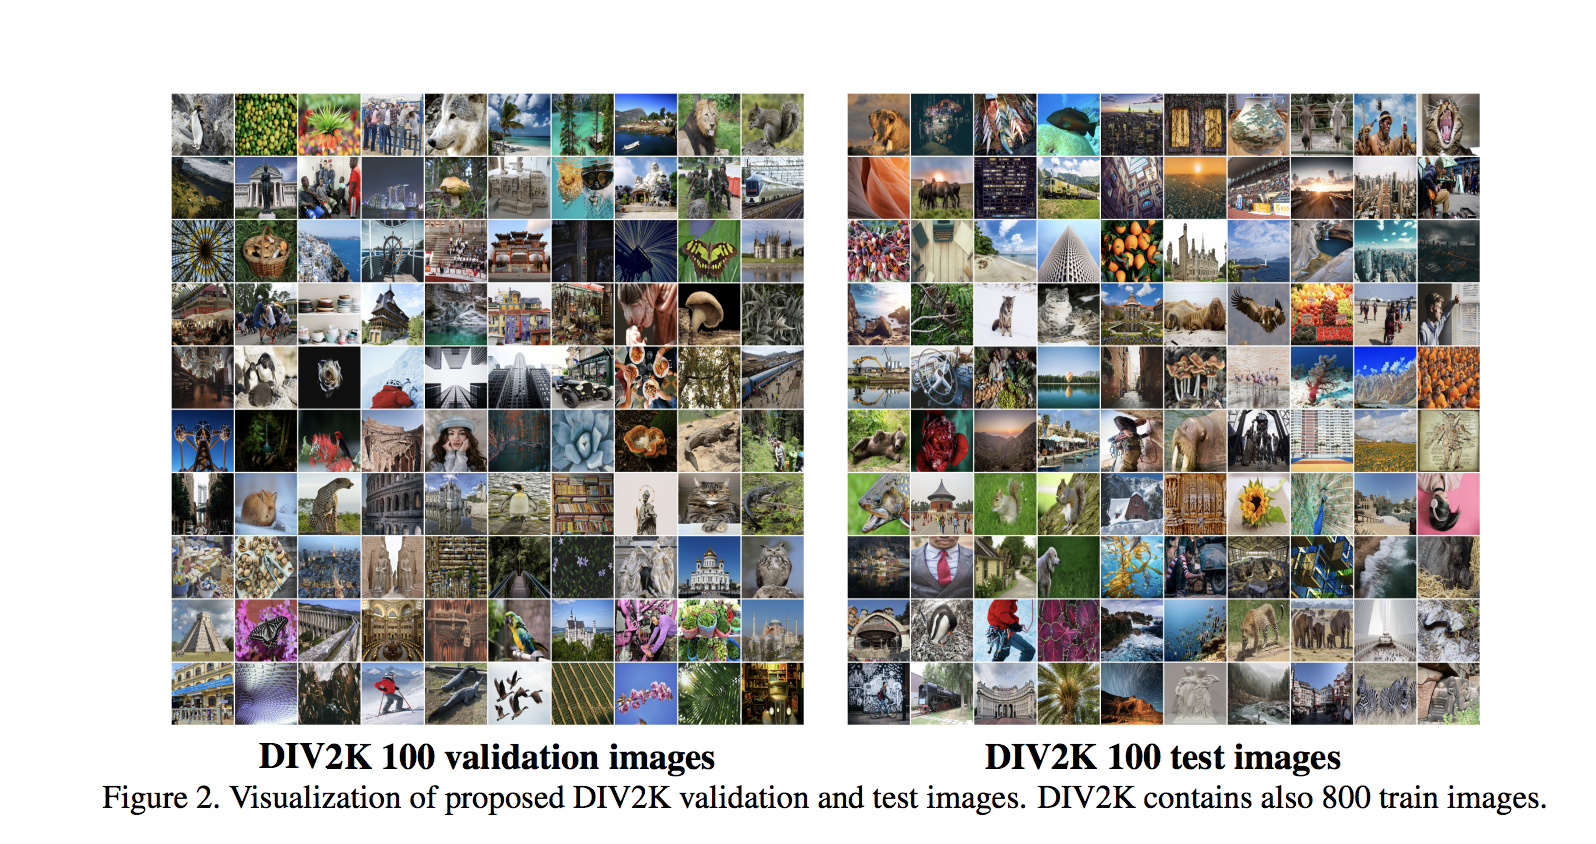
\includegraphics[width=13cm]{imgs.png}
\end{figure}

  \item \textbf{What software/hardware will you use?}
  
  In order to take advantage of past experience and debugging help from course staff, we will likely choose an infrastructure such as TensorFlow that has a large community of users who have demonstrated good super-resolution results previously.  We will need to have some significant compute power and testing infrastructure to train our model. We would like to explore using the Brown CCV High Performance Computing Cluster or credits on Google Cloud Platform in order to train our model. 
  
  \item \textbf{What are the skills of the team members? Who will do what?}
  
  \textbf{Gabe:} I have experience with Tensorflow, so if we go with a learning based approach I can handle implementing the model. I also have experience building GUIs in Python. If we choose to make a GUI for this project I would handle that. 
  
  \textbf{Mary:} I took Deep Learning last semester so I also have experience with Tensorflow and GANs. I would help with preprocessing the data and building the model. I would also do more research into state-of-the-art methods and share notes with the group.

  \textbf{Michael} Most of my experience with machine learning and computer vision are in this class. I will research and implement other approaches to solve the problem that do not use machine learning, such as the application of filters for sharpening.
  
  \textbf{Peter} I took AI last semester and have a bunch of experience with web-servers and web front-ends if we decide to implement a web-app of some sort.  
  
  \item \textbf{How will you know whether you have made progress? What will you measure?}
  
  Once we have the algorithm working at a basic level, assessing progress will be mostly subjective. We will mostly likely rely on looking at the output images to see how ``good" they look. Comparing the output of our algorithm to the output of a less intelligent method, such as a simple sharpening filter, will provide a good reference for our assessments.
  
  A more objective measure that we could use for benchmarking different implementations would be to see how much an image of text can be downsampled before the re-upsampled version becomes unreadable. A similar test could be done with faces to see how much downsampling can be done before the person is no longer recognizable. 
  
  To compare our model to state-of-the-art algos quantitatively, we can also use the NTIRE's open-source Image Quality Assessment script. This script scores the output of our model using Mean-Squared Error and Peak Signal-to-Noise Ratio. Link at the bottom of \href{https://data.vision.ee.ethz.ch/cvl/DIV2K/}{this page}.
 
  \item \textbf{What problems do you foresee or have?}
  
  One potentially difficult aspect of this project, especially for a learning based approach, will be allowing the input image to be of variable size. Though a having a fixed input size may be acceptable, it would limit the usefulness of the algorithm and we would like to avoid this constraint.
  
  Besides that, the biggest danger with a learning based approach will be keeping training time reasonable. This will depend heavily on the level of hardware that we have access to. 

  \item Is there anything that we can do to help? E.G., resources, equipment.
  
  We've noticed that some of the course staff are especially well versed in machine learning and think that we could benefit from tips regarding the architecture for the neural network we will build, or a hint on what existing architecture we can leverage for this project. 
  
  Since we are considering training a network to upscale the images, and we will likely need to use large image files, the use of a powerful computer would be important to let us train the network in a reasonable amount of time. We would appreciate access to the CIT's computing cluster. We also have some remaining credit left on GCP, but might run out if we decide to use it for this project.
 
  \item \textbf{References}
  
  \url{www.igl.ethz.ch/projects/prosr/}
  
  \url{https://data.vision.ee.ethz.ch/cvl/DIV2K/}
  
  \url{www.vision.ee.ethz.ch/~timofter/publications/Agustsson-CVPRW-2017.pdf}
  
\end{itemize}


\end{document}
